\chapter{Project description}
\ifpdf
    \graphicspath{{Chapter2/PNG/}{Chapter2/PDF/}{Chapter2/}}
\else
    \graphicspath{{Chapter2/Chapter2Figs/EPS/}{Chapter2/}}
\fi

This internship is taken place within the project Bipop whose research topic is the study of
nonsmooth dynamical systems. It is part of a collaboration with the company
Trasys contracting the European Space Agency (ESA), in particular, has developed a Trasys
3D simulation software of a Mars Rover: 3DROV. Bipop develops a software platform SICONOS for
simulation of nonsmooth dynamic systems, especially mechanical systems. Better friction-contact models could be involved in Siconos to improve the existing simulation in 3DROV\\

The objective of the course internship is to integrate the simulation engine in the tool SICONOS
visualization 3DROV ESA and test simulations of moving a Rover Mars on a granular soil.

\begin{figure}[H]
 \begin{center}
      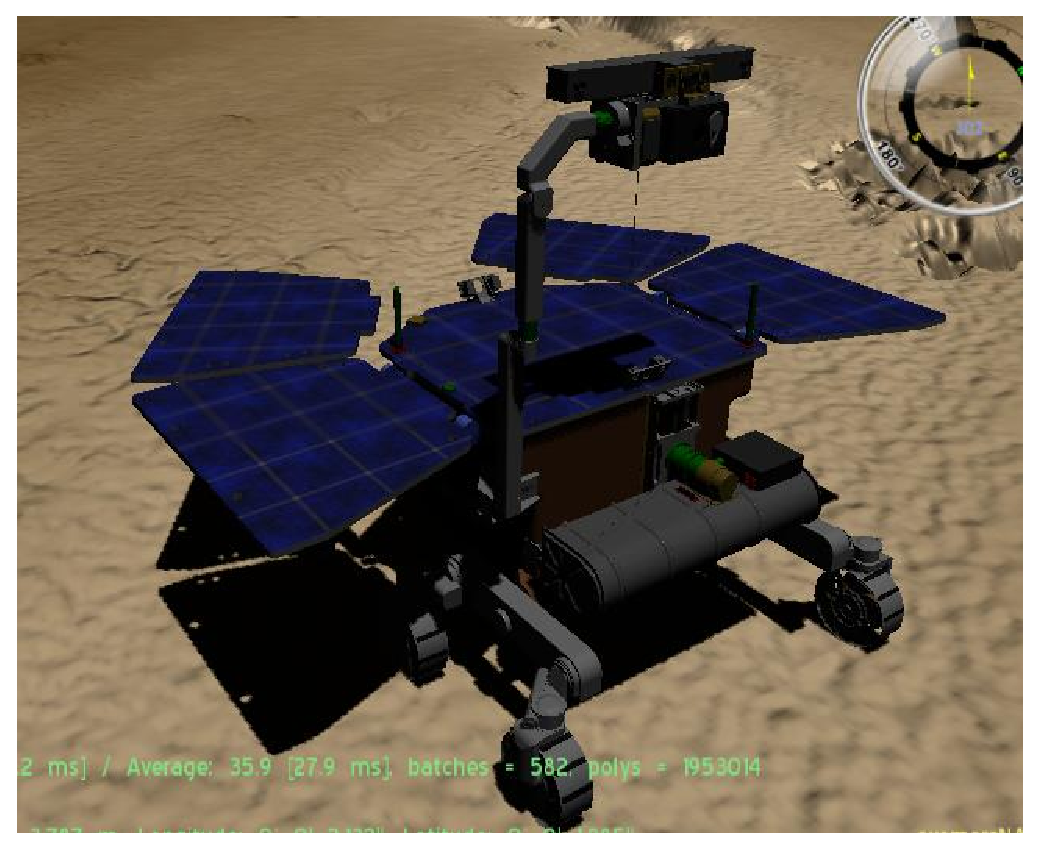
\includegraphics[width=8cm]{stage.EPS}
  \end{center}
\end{figure}


The main objectives of the internship are:

\begin{itemize}
\item Learning to use the platform SICONOS, dynamics and non-regular
models of contact friction
\item Create a 2D model to simulate Rover on granular soil.
\item Implement a Maple code to generate the dynamical system automatically for 3D Rover
\item Make simulation for the 3D Rover model on granular soil.
\item Learning the API viewer 3DROV.
\item Specification in conjunction with Trasys integration of simulation engine in SICONOS
3DROV coding and integration.
\item Experimental simulation of the rover on a granular soil.
\item Implement methods of time integration and the sliding contact.
\end{itemize}

